\documentclass{beamer}
\definecolor{envy}{HTML}{1A936F}
%\definecolor{berry}{HTML}{C6878F}
\definecolor{berry}{HTML}{A0747A}
\definecolor{turq}{HTML}{077187}
%\definecolor{pgreen}{HTML}{CBE896}
\definecolor{pgreen}{HTML}{D9D0DE}
\definecolor{db}{HTML}{1D3461}
\colorlet{ldb}{db!55!white}
\colorlet{lpgreen}{pgreen!55!white}

\newcommand{\light}[1]{\textcolor{db!50!white}{#1}}
% New colours!
% \setbeamercolor{background canvas}{bg=GreyWhite}

\setbeamercolor{title}{fg=db, bg=pgreen!55!white}
\setbeamercolor{frametitle}{fg=db, bg=pgreen!55!white}
\setbeamercolor{normal text}{fg=db}
\setbeamercolor{block title}{fg=db,bg=pgreen!55!white}
%%\setbeamercolor{title}{fg=black, bg=pgreen!55!white}
%%\setbeamercolor{frametitle}{fg=black, bg=pgreen!55!white}
%%\setbeamercolor{normal text}{fg=black}
%%\setbeamercolor{block title}{fg=black,bg=pgreen!55!white}
%%\setbeamercolor{block body}{fg=black!22!white}
%\setbeamercolor{alerted text}{fg=Pinky}
\setbeamercolor{itemize item}{fg=db!85!white}
\setbeamercolor{itemize subitem}{fg=db!85!white}
\setbeamercolor{itemize subsubitem}{fg=db!85!white}
%\setbeamercolor{framesource}{fg=Carrot}
%\setbeamercolor{section in toc}{fg=PurpNav}
\setbeamercolor{footnote}{fg=black}
\setbeamercolor{footnote mark}{fg=black}
\setbeamercolor{myfootlinetext}{fg=black}
\setbeamertemplate{itemize subitem}{fg=turq}
\setbeamertemplate{itemize subsubitem}{fg=turq}
%\setbeamertemplate{itemize item}{\color{DarkPurple}$\blacksquare$}
%\setbeamertemplate{itemize item}{\color{DarkPurple}}[circle]
\setbeamertemplate{itemize item}[circle]

\newcommand{\be}{\begin{enumerate}}
	\newcommand{\ee}{\end{enumerate}}
\newcommand{\bi}{\begin{itemize}}
	\newcommand{\ei}{\end{itemize}}
\newcommand{\ccbb}{\cellcolor{turq!15!white}}
\newcommand{\cc}{\cellcolor{pgreen!55!white}}
\newcommand{\ccb}{\cellcolor{berry!35!white}}

% source at bottom left of slide
\newcommand{\sourceleft}[1]{\begin{textblock*}{4cm}(0.3cm,8.8cm)
		\begin{beamercolorbox}[ht=0.5cm,left]{framesource}
			\usebeamerfont{framesource}\usebeamercolor[fg]{framesource}
			{#1}
		\end{beamercolorbox}
	\end{textblock*}}
	
% source at bottom right of slide
\newcommand{\sourceright}[1]{\begin{textblock*}{}
		\begin{beamercolorbox}[ht=0.5cm,left]{framesource}
			\usebeamerfont{framesource}\usebeamercolor[berry]{framesource}
			{#1}
		\end{beamercolorbox}
	\end{textblock*}}

\newcommand{\cfcite}[1]{\footnote{\citeauthor{#1}, \citeyear{#1}}}

\newcommand{\sourceextremeright}[1]{\begin{textblock*}{4cm}(10.6cm,8.8cm)
		\begin{beamercolorbox}[ht=0.5cm,left]{framesource}
			\usebeamerfont{framesource}\usebeamercolor[fg]{framesource}
			{#1}
		\end{beamercolorbox}
	\end{textblock*}}

\usetheme{boxes}
\usepackage[absolute,overlay]{textpos}
%\usecolortheme{beaver}
\useinnertheme{circles}
\usepackage{amsmath}
\usepackage{amssymb}
\usepackage{lmodern}
\usepackage{xcolor}
\usepackage{tikz-cd}
\usepackage{tikz}
\usepackage{beamerthemesplit} %for the pause on the quad slide?
\usetikzlibrary{arrows.meta}
\usetikzlibrary{decorations.markings}
\usetikzlibrary{calc, arrows}
\usepackage{longtable}
\usepackage{graphicx}% http://ctan.org/pkg/graphicx
\usepackage{booktabs}
\usepackage{xspace}
\usepackage{varwidth}
\usepackage{array} %make columns all same width
%\newcolumntype{C}{>{\centering\arraybackslash}p{0.2\linewidth}}
%\usepackage{scrtime} % for \thistime (this package MUST be listed first!)
\usepackage{amsmath} % essential for cases environment
\usepackage{amsthm} % for theorems and proofs
\usepackage{amsfonts} % mathbb
\usepackage{graphics,graphicx}
\usepackage{multirow} % fancy tables
\usepackage{wasysym} % circle symbols (including half-filled circles)
\usepackage{enumerate} % fancier enumeration (e.g., a,b,c, ...)
%\usepackage{xcolor}
\usepackage{color}
\usepackage{xstring}
\usepackage[linguistics]{forest}
\usetikzlibrary{calc, arrows}
\usepackage{xcolor,colortbl}
\usepackage[export]{adjustbox}
\usepackage{lipsum}
\usepackage{calc}
\usepackage{array} %to uncover one col at a time of a table
%\colorlet{grey}{black!10}
%below adds slide number without putting total number of slides
\setbeamertemplate{footline}{%
	\raisebox{8pt}{\makebox[\paperwidth]{\hfill\makebox[10pt]{\scriptsize\insertframenumber}}}}

\newenvironment{itmenv}{\only{\setbeamercolor{local structure}{fg=gray}}}{}
\setbeamertemplate{enumerate items}[default]
\setbeamercolor*{enumerate item}{fg=db}

\setbeamercolor*{enumerate subitem}{fg=db}
\newcommand\FrameText[1]{%
	\begin{textblock*}{\paperwidth}(0pt,\textheight)
		\raggedleft #1\hspace{4em}\vspace{20em}
	\end{textblock*}}

\mode<presentation>
\title{\Huge Visualizing Molecular Trends in Bacterial Genomes}

\author[Daniella Lato]{\\ \textbf{Daniella Lato and Jana Taha}\\ Stats 744: Final Project\\ December 3, 2019}
\date[2017]{}
\IfFileExists{upquote.sty}{\usepackage{upquote}}{}
\newcommand{\itm}{\item<itm@1->}
\newcommand{\btVFill}{\vskip0pt plus 1filll}
\newcommand{\s}{\textit{Sinorhizobium}\ }
\newcommand{\sm}{\textit{Sinorhizobium meliloti}\xspace}
\newcommand{\salm}{\textit{Salmonella enterica}\xspace}
\newcommand{\smel}{\textit{S.\,meliloti}\xspace}
\newcommand{\smed}{\textit{S.\,medicae}}
\newcommand{\sfred}{\textit{S.\,fredii}}
\newcommand{\ssah}{\textit{S.\,saheli}}
\newcommand{\ster}{\textit{S.\,terangae}}
\newcommand{\ag}{\textit{Agrobacterium tumefaciens }}
\newcommand{\p}{progressiveMauve\xspace}
\newcommand{\agro}{\textit{A.\,tumefaciens }}
\newcommand{\bur}{\textit{Burkholderia}\xspace}
\newcommand{\vib}{\textit{Vibrio}\xspace}
\newcommand{\bor}{\textit{Bordetella}\xspace}
\newcommand{\xan}{\textit{Xanthomonas}\xspace}
\newcommand{\sul}{\textit{Sulfolobus}\xspace}
\newcommand{\ent}{\textit{Enterobacteria}\xspace}
\newcommand{\bac}{\textit{Bacillus subtilis}\xspace}
\newcommand{\ecoli}{\textit{Escherichia coli}\xspace}
\newcommand{\lis}{\textit{Listeria monocytogenes}\xspace}
\newcommand{\bass}{\textit{B.\,subtilis}\xspace}
\newcommand{\bas}{\textit{Bacillus subtilis}\xspace}
\newcommand{\tub}{\textit{Mycobacterium tuberculosis}\xspace}
\newcommand{\strep}{\textit{Streptomyces}\xspace}
\newcommand{\agrot}{\textit{Agrobacterium tumefaciens}\xspace}
\newcommand{\ecol}{\textit{E.\,coli}\xspace}
\newcommand{\salb}{\textit{S.\,alblus}\xspace}
\newcommand{\salbus}{\textit{S.\,albus}\xspace}
\newcommand{\shyg}{\textit{S.\,hygroscopicus}\xspace}
\newcommand{\sliv}{\textit{S.\,lividans}\xspace}
\newcommand{\sros}{\textit{S.\,roseosporus}\xspace}
\newcommand{\ssir}{\textit{S.\,sirex}\xspace}
\newcommand{\sven}{\textit{S.\,venezuelae}\xspace}
\newcommand{\scoe}{\textit{S.\,coelicolor}\xspace}
\newcommand{\hal}{\textit{Haloquadratum walsbyi}\xspace}
\newcommand{\pa}{pSymA\xspace}
\newcommand{\pb}{pSymB\xspace}
\newcommand{\ch}{$\checkmark$}
\setbeamertemplate{navigation symbols}{}
\newcommand*{\NodeSize}{0.5cm}%
\newcommand*{\YShiftBetweenRows}{-1cm}% Subsequent rows are shited down so they don't overlap
%\tikzset{DNA Style/.style={minimum size=0.5cm, draw=gray, line width=1pt}}{}
\providecommand{\e}[1]{\ensuremath{\times 10^{#1}}}
\newlength{\YShift}% 
\newcounter{ColumnCounter}% Prefix for node labels

\newcommand\FourQuad[4]{%
	\begin{minipage}[b][.35\textheight][t]{.47\textwidth}#1\end{minipage}\hfill%
	\begin{minipage}[b][.35\textheight][t]{.47\textwidth}#2\end{minipage}\\[0.5em]
	\begin{minipage}[b][.35\textheight][t]{.47\textwidth}#3\end{minipage}\hfill
	\begin{minipage}[b][.35\textheight][t]{.47\textwidth}#4\end{minipage}%
}

% Initialize - These are probably not needed, but prefer to set them
\setlength{\YShift}{0cm}% 
\setcounter{ColumnCounter}{0}


%%%%%%%%%%%%%%%%%%%%%%%%%%%%%%%%%%%%%%%%%%%%%%%%%%%%%%%%%%%%%%%%%%%%%%%%%%%%%%%%%%%%%%%%%%%%%%%%%%%%%%%%%%%%%%%%%%%%%%%%%%%%%%%%%%%%%%%%%%%%%%%%%%%%%%%%%%%%%%%%


\begin{document}
% \titlegraphic{text} %for including logos in title. have to adjust vspace and hspace	
	\begin{frame}
		
		\titlepage
		
	\end{frame}
	%\begin{frame}
	%\begin{center}
	
	%\huge{Introduction}
	
	%\end{center}
	%\end{frame}
%%%%%%%%%%%%%%%%%%%%%%%%%%%%%%%%%%%%%%%%%%%%%%%%%%%%%%%
\begin{frame}{The Organisms}
	Bacteria:
	\bi
	\itm \ecoli
	\itm \bas
	\itm \strep
	\itm \sm
	\ei
	\vfill
	
	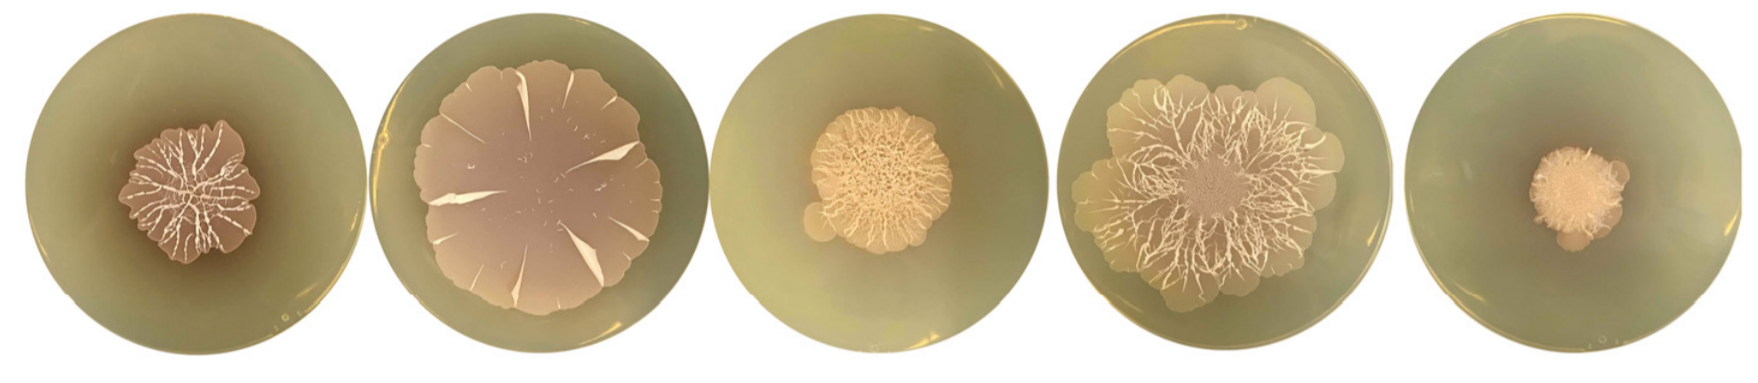
\includegraphics[width=\textwidth]{strep_pic}
%\begin{figure}
%	\hfill\begin{minipage}{.5\textwidth}\centering
%		\includegraphics[scale=0.4]{smel_pic}
%		
\centering
		{\centering \tiny Photo: \strep by Stephanie Jones, McMaster University}
%		%		\caption{\texttt{minipage}}
%	\end{minipage}
%\end{figure}
\end{frame}
%%%%%%%%%%%%%%%%%%%%%%%%%%%%%%%%%%%%%%%%%%%%%%%%%%%%
\begin{frame}[t]{Biological Background}
	\bigskip
	\begin{columns}[t]
		\column{0.30\textwidth}
		\textbf{1) Circular}
		\centering
		\begin{tikzpicture}
		%circle
		\draw[thick] (4,0) circle (1cm);
		%origin tick
		\draw[thick] (4,0.8) -- (4,1.2);
		\tikzstyle{none}=[draw = none, minimum width=2cm, minimum height=0.3cm, rounded corners]
		\node[none] (first reservoir) at (4,-4) {\ecoli};
		\tikzstyle{ntwo}=[draw = none, minimum width=2cm, minimum height=0.3cm, rounded corners]
		\node[ntwo] (second reservoir) at (4,-4.5) {\bas};
		\end{tikzpicture}
		
		\column{0.30\textwidth}
		\textbf{2) Linear}
		\centering
		
		\bigskip
		\begin{tikzpicture}
	%line
		\draw[thick] (3.5,0) -- (6.5,0);
		%origin tick
		\draw[thick] (4.5,-.2) -- (4.5,.2);
		\tikzstyle{none}=[draw = none, minimum width=2cm, minimum height=0.3cm, rounded corners]
		\node[none] (first reservoir) at (5,-5.1) {\strep};
		\end{tikzpicture}
		
		\column{0.4\textwidth}
		\textbf{3) Multi-repliconic}
		\centering
		\begin{tikzpicture}
		%chrom
		\draw[thick] (0,0) circle (1cm) node {\tiny Chromosome};
		%ori tick
		\draw[thick] (0,0.8) -- (0,1.2);
		%pSymA
		\draw[thick] (0,-1.75) circle (0.5cm) node {\tiny \pa};
	%ori tick
		\draw[thick] (0,-1.1) -- (0,-1.4);
		%pSymB
		\draw[thick] (0,-3.25) circle (0.75cm) node {\tiny \pb};
		%ori tick
		\draw[thick] (0,-2.35) -- (0,-2.65);
		\tikzstyle{none}=[draw = none, minimum width=2cm, minimum height=0.3cm, rounded corners]
		\node[none] (first reservoir) at (0,-4.5) {\sm};
		\end{tikzpicture}
	\end{columns}
\end{frame}
%%%%%%%%%%%%%%%%%%%%%%%%%%%%%%%%%%%%%%%%%%%%%%%%%%%
%%%%%%%%%%%%%%%%%%%%%%%%%%%%%%%%%%%%%%%%%%%%%%%%%%%%
\begin{frame}[t]{Bacterial Genome Properties}
	\begin{columns}[t]
		\begin{column}{0.5\textwidth}
	Bidirectional Replication
		\bi
		\itm Gene dosage
		\itm Sequence composition
		\itm Codon bias
		\itm Replication errors
		\itm Strand differences
		\ei
	\bigskip
	
		\centering{
			\resizebox{\textwidth}{!}{%
				\begin{tikzpicture}
			
	%new DNA label
	\node[berry] at (0.15,-2) {\fontsize{1}{1}\selectfont \textbf{-- new DNA}};
	%old DNA label
	\node[] at (0.15,-2.05) {\fontsize{1}{1}\selectfont \textbf{-- old DNA}};
				\end{tikzpicture}
			}%resiebox
		}%centering
\end{column}
\begin{column}{0.5\textwidth}
%	\centering{
%		\resizebox{\textwidth}{!}{%
%			\begin{tikzpicture}
%			%fig lable A
%			\node[berry] at (0,0) {\fontsize{10}{3}\selectfont \textbf{-- new DNA}};
%			\end{tikzpicture}
%		}%resiebox
%	}%centering
		\centering{
			\resizebox{\textwidth}{!}{%
				\begin{tikzpicture}[x=0.5cm, y=0.5cm]
				\tikzstyle{neleven}=[draw = none, minimum width=0.05cm, minimum height=0.05cm, berry]
				%new DNA label
%				\node[neleven] at (0.15,-3) {\fontsize{1}{1}\selectfont \textbf{-- new DNA}};
%				\draw[line width=0.01mm,
%				postaction={decorate}, fill=black] (0,-2.5) circle (0.008cm);
%				\draw[line width=0.01mm,
%				postaction={decorate}, fill=pink] (0.15,-2.9) circle (0.008cm);
				%%% TOP CIRCLE %%%
				%rep bubble circle
%				\draw[line width=0.01mm,
%				postaction={decorate}] (0,-2.3) ellipse (0.05cm and 0.02cm);
				%old DNA outter circle
				\draw[line width=0.05mm,
				postaction={decorate}] (0,-2.5) circle (0.1cm);
				%old DNA top arc
				\draw[line width=0.05mm] (0.153,-2.4) arc (-80:-100:0.44cm);
				%old DNA bottom arc
				\draw[line width=0.05mm] (0.15,-2.4) arc (30:-210:0.086cm);
				%new DNA top arc
				\draw[line width=0.05mm, berry] (0.136,-2.383) arc (40:140:0.09cm);
				%new DNA bottom arc
				\draw[line width=0.05mm, berry] (0.136,-2.38) arc (-80:-100:0.394cm);
				%old DNA inner circle
%				\draw[line width=0.01mm,
%				postaction={decorate}] (0,-2.5) circle (0.09cm);
				%arrow inbtwn circles
				\draw[-{Latex[width=0.1mm,length=0.2mm]},line width = 0.03mm] (0,-2.72) -- (0,-2.79);
				%%% BOTTOM CIRCLE %%%
				%old DNA outter circle
				\draw[line width=0.05mm,
				postaction={decorate}] (0,-3) circle (0.1cm);
%				%old DNA inner circle
%				\draw[line width=0.01mm,
%				postaction={decorate}] (0,-3) circle (0.09cm);
				%old DNA bottom arc
				\draw[line width=0.05mm] (0.15,-2.9) arc (0:-180:0.0748cm);
				%old DNA Inner arc
				\draw[line width=0.05mm] (0.15,-2.9) arc (30:-210:0.086cm);
				%new DNA top arc
				\draw[line width=0.05mm, berry] (0.1369,-2.882) arc (40:140:0.089cm);
				%new DNA bottom arc
				\draw[line width=0.05mm, berry] (0.1369,-2.881) arc (0:-180:0.068cm);
				%arrow for rep to the right
				\draw[-{Latex[width=0.1mm,length=0.2mm]},line width = 0.03mm] (0.05,-2.881) -- (0.13,-2.881);
				%arrow for rep to the left
				\draw[-{Latex[width=0.1mm,length=0.2mm]},line width = 0.03mm] (-0.05,-2.881) -- (-0.13,-2.881);

				\end{tikzpicture}
			}%resiebox
		}%centering


	\end{column}
\end{columns}
	\btVFill
		\tiny \vspace{-\baselineskip}\color{berry}{Rocha 2004, Quax et al. 2015, Hyrien et al. 2013}
\end{frame}

%%%%%%%%%%%%%%%%%%%%%%%%%%%%%%%%%%%%%%%%%%%%%%%%%%%
%%%%%%%%%%%%%%%%%%%%%%%%%%%%%%%%%%%%%%%%%%%%%%%%%%%%%%%
\begin{frame}{Bacterial Genomes}
\Large
\centering
	Different \textbf{replicons} and \textbf{positions} of bacterial genomes can have \textbf{varying molecular trends}
	
	
\end{frame}

%%%%%%%%%%%%%%%%%%%%%%%%%%%%%%%%%%%%%%%%%%%%%%%%%%%%

\begin{frame}{Spatial Molecular Trends}
	\begin{columns}[t]
		\column{.5\textwidth}
		\centering
		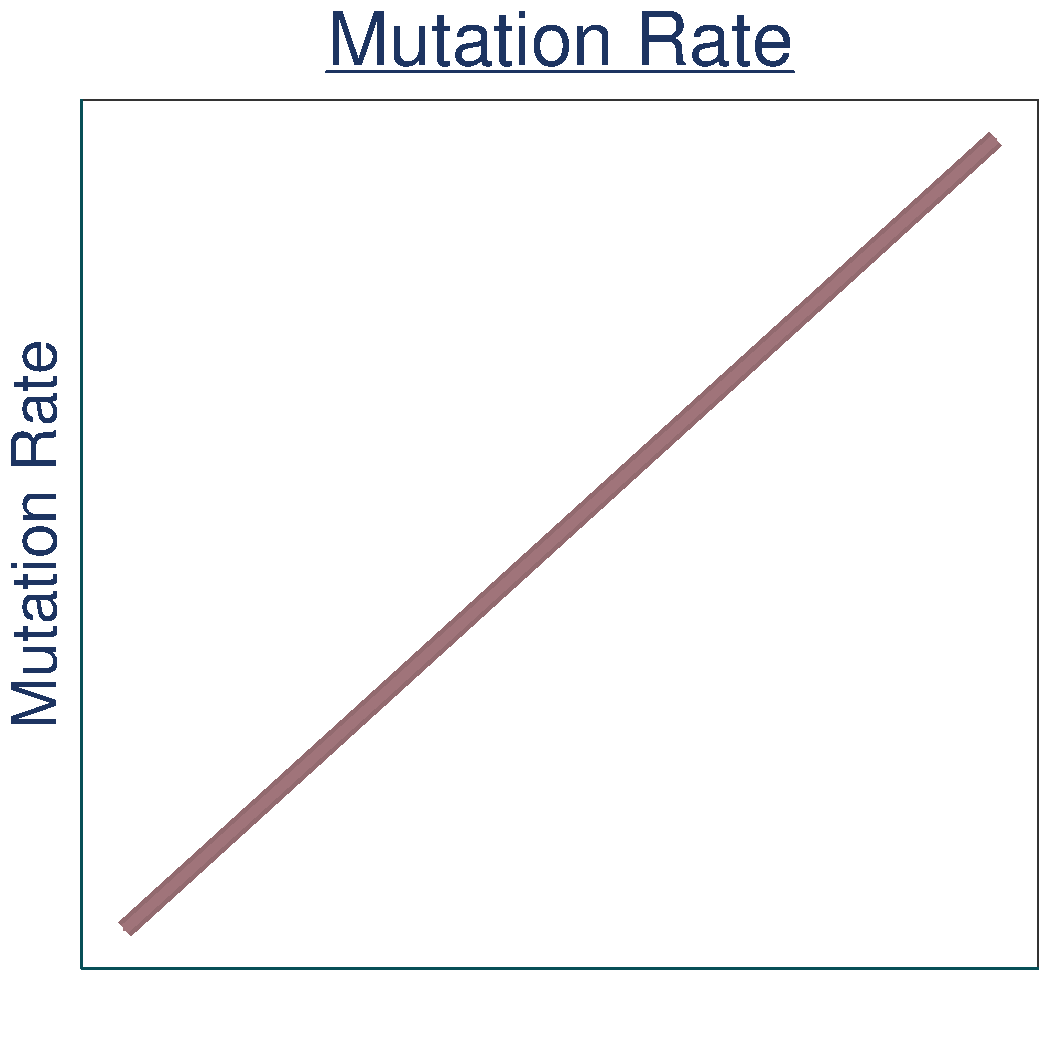
\includegraphics[width=0.67\textwidth]{./mut_graph.pdf}\\
		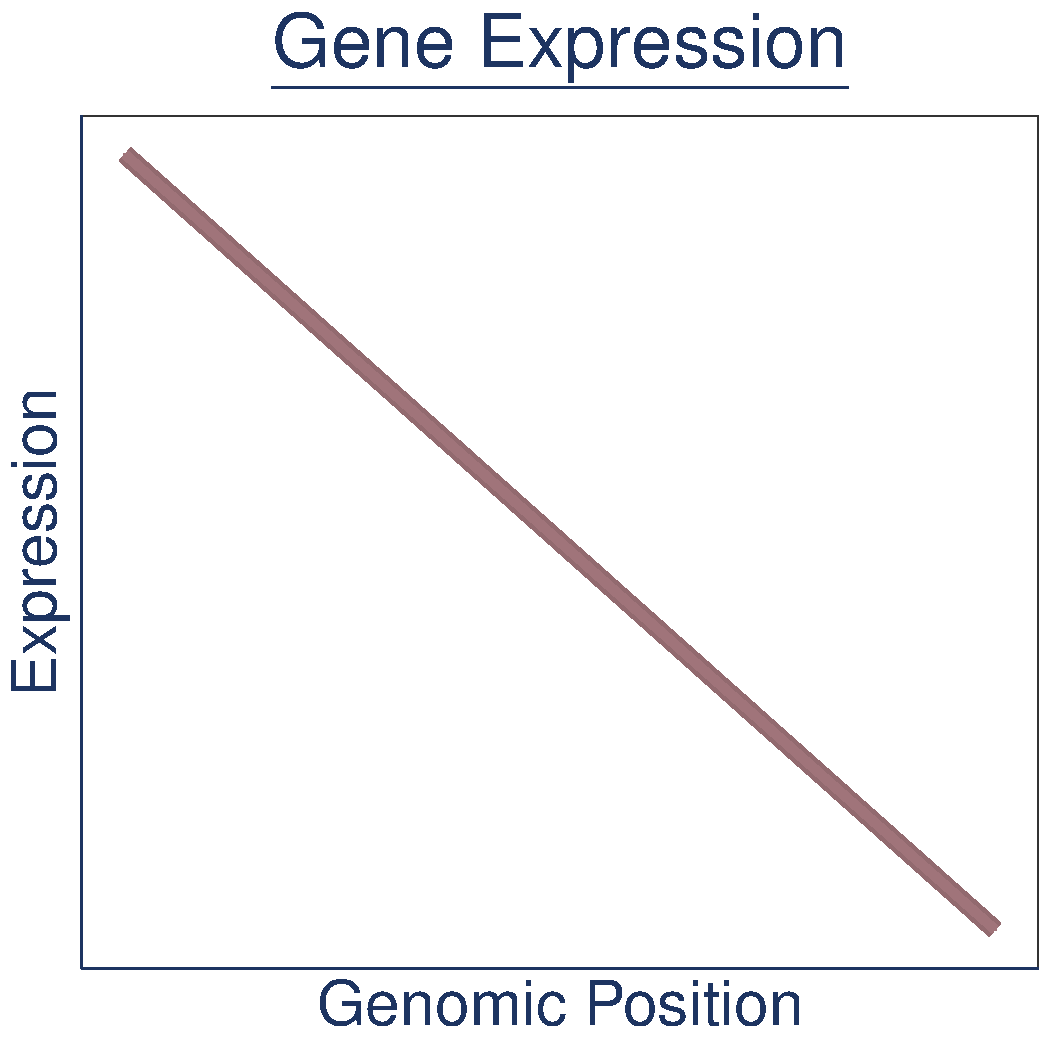
\includegraphics[width=0.67\textwidth]{./exp_graph.pdf}
		\column{.5\textwidth}
		\centering
		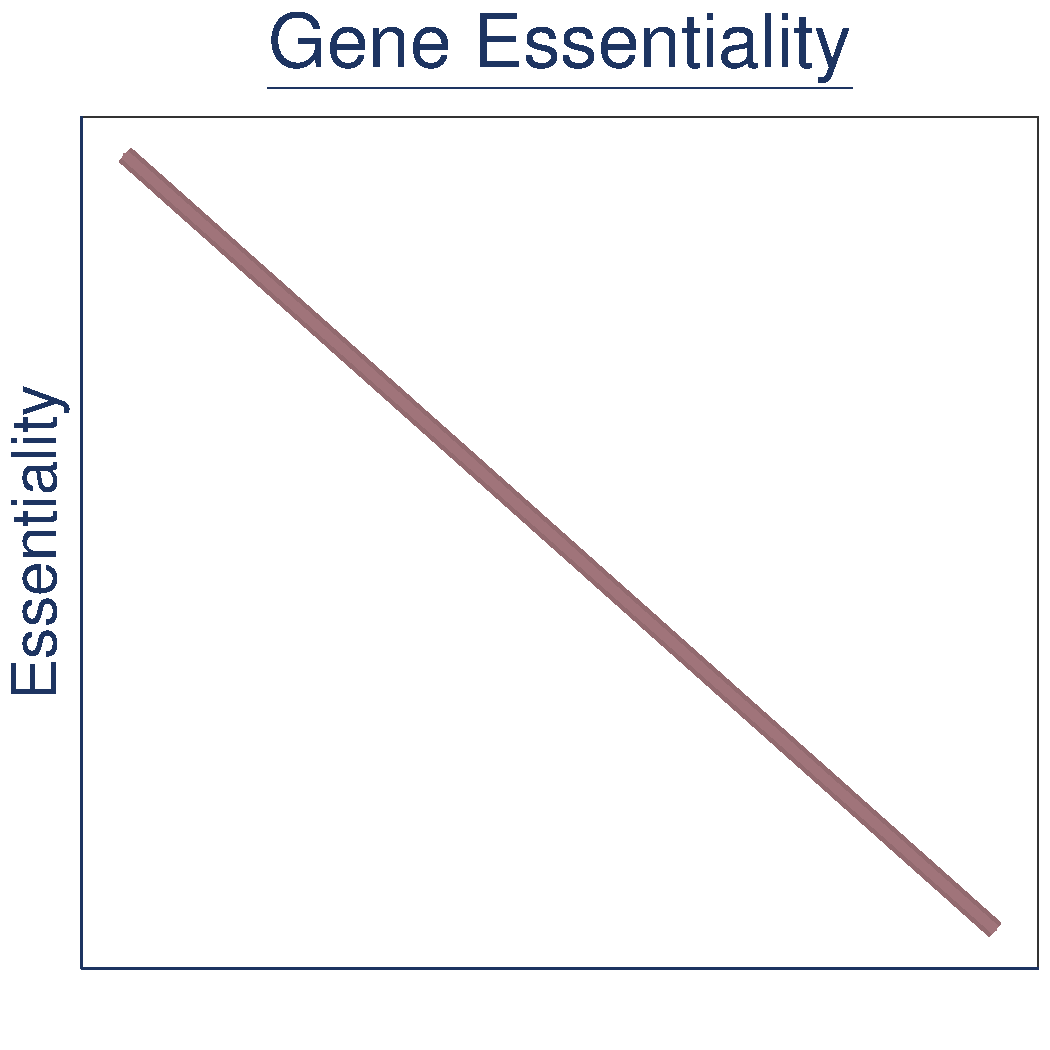
\includegraphics[width=0.67\textwidth]{./ess_graph.pdf}\\
		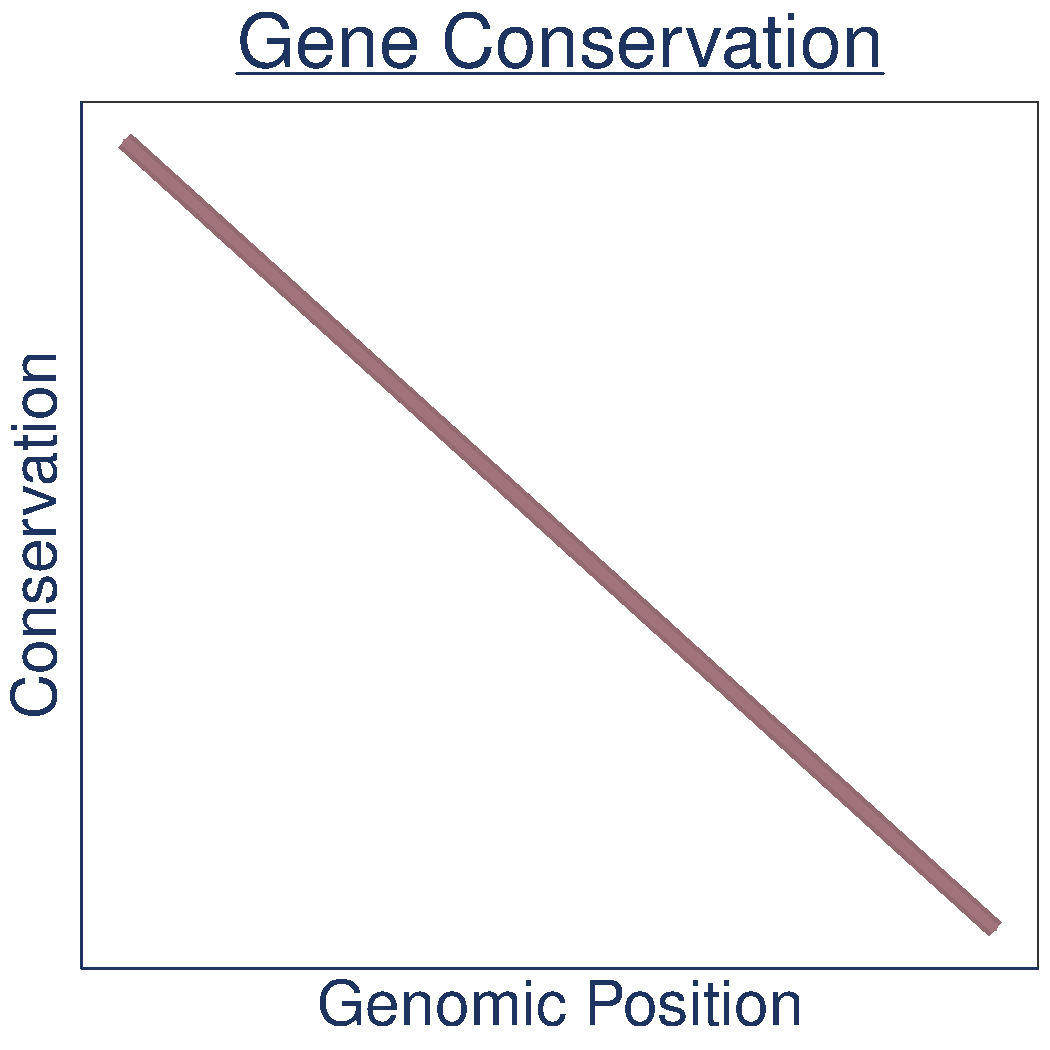
\includegraphics[width=0.67\textwidth]{./cons_graph.pdf}
	\end{columns}
	
	\btVFill
	\tiny \vspace{-\baselineskip}\color{berry}{Couturier et al. 2006, Cooper et al. 2010, Sharp et al. 2005, Morrow et al. 2012, Cooper and Rocha 2006}
	%		\sourceright{Couturier et al. 2006, Cooper et al. 2010, Sharp et al. 2005, Morrow et al. 2012, Cooper and Rocha 2006}
	
\end{frame}
%%%%%%%%%%%%%%%%%%%%%%%%%%%%%%%%%%%%%%%%%%%%%%%%%%%
\begin{frame}[t]{The Data}
	\textbf{Gene Expression}
	\bi
	\itm \ecol, \bass, \strep, and \smel
	\itm Gene expression + distance from the origin of replication
	\itm \textbf{Expectation:} Near the origin or replication = Higher Expression
	\ei
	
	\bigskip
	
	We will focus on \strep
	
\end{frame}
%%%%%%%%%%%%%%%%%%%%%%%%%%%%%%%%%%%%%%%%%%%%%%%%%%
\begin{frame}{Gene Expression}
	\centering
	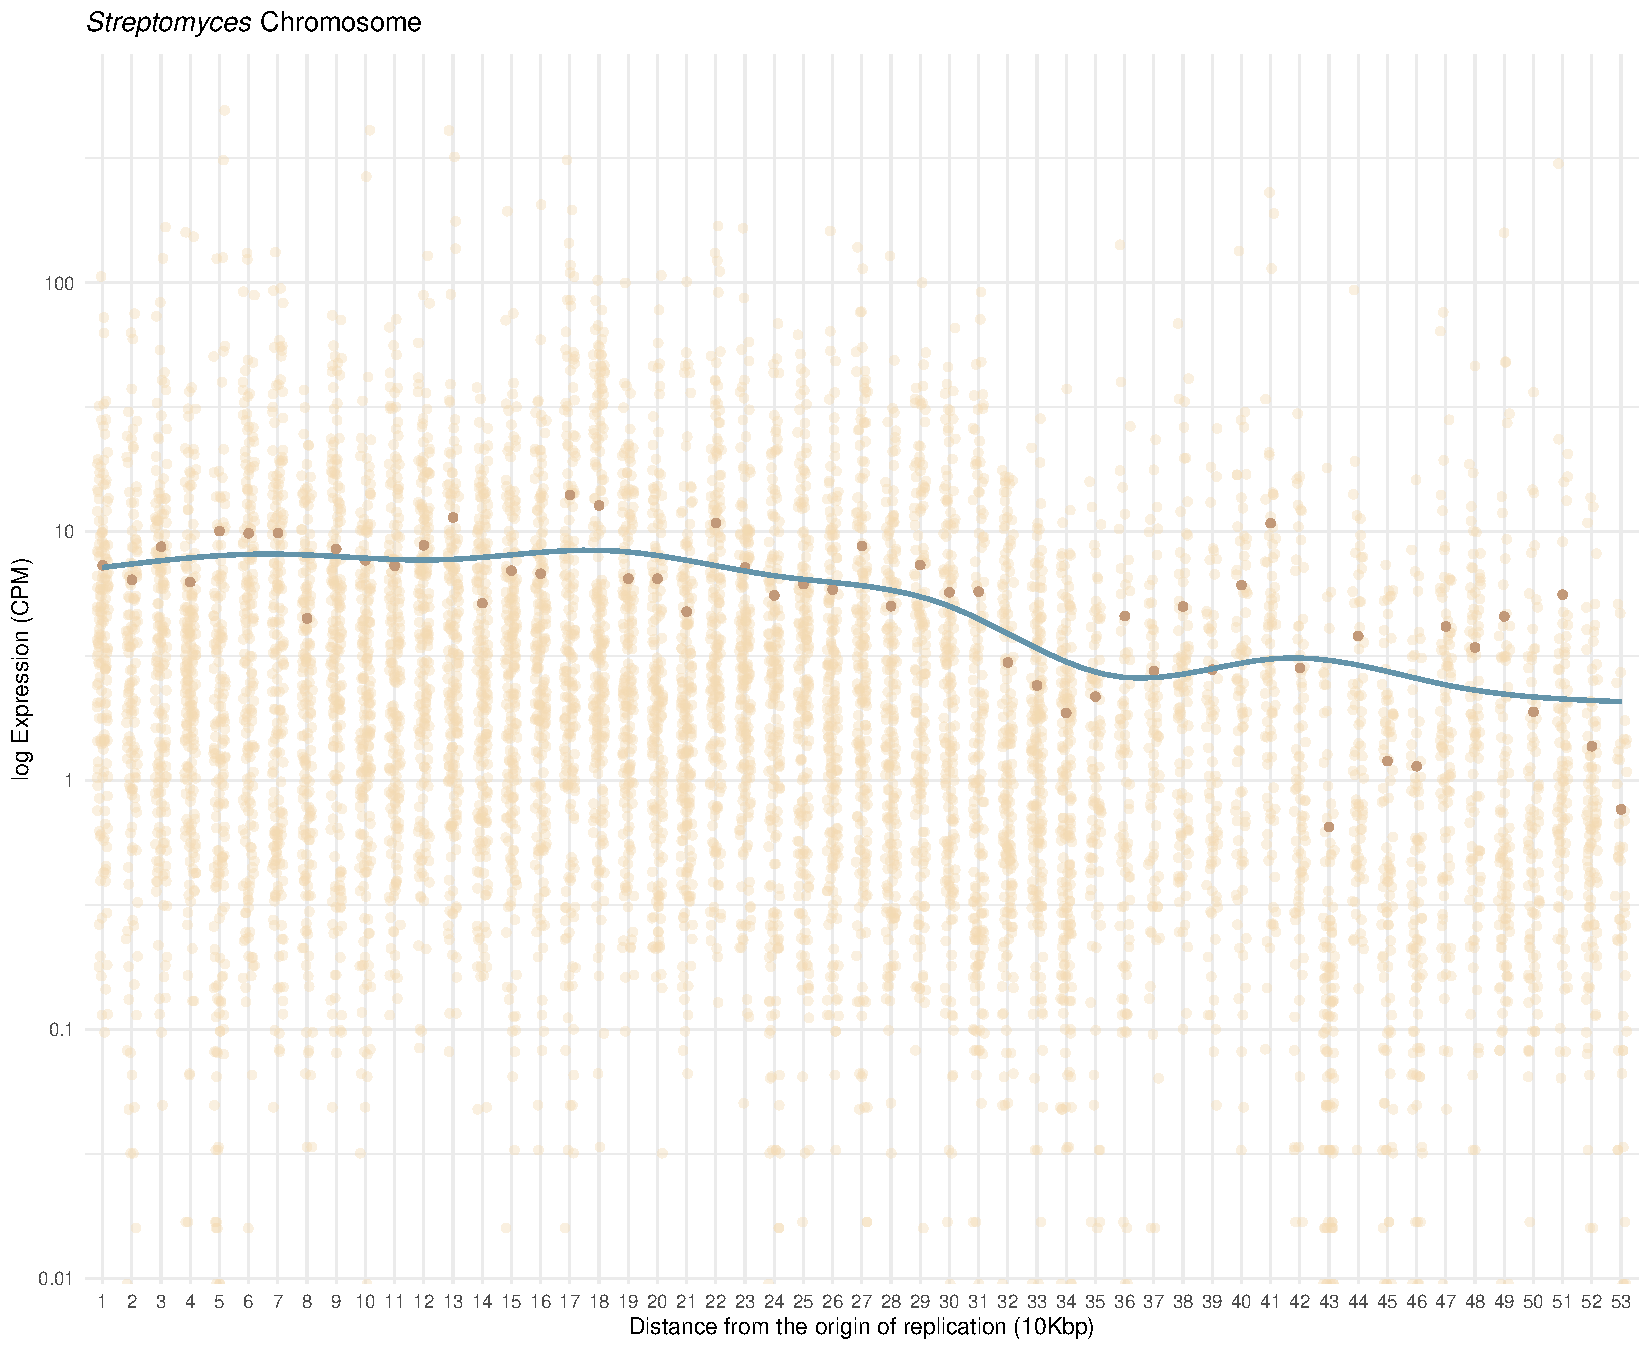
\includegraphics[width=0.95\textwidth]{strep_expression_plot.pdf}
\end{frame}
%%%%%%%%%%%%%%%%%%%%%%%%%%%%%%%%%%%%%%%%%%%%%%%%%%
%%%%%%%%%%%%%%%%%%%%%%%%%%%%%%%%%%%%%%%%%%%%%%%%%%%%

\begin{frame}{Spatial Molecular Trends}
	\begin{columns}[t]
		\column{.5\textwidth}
		\textbf{Expectation: }
		\centering
		\bigskip
		
		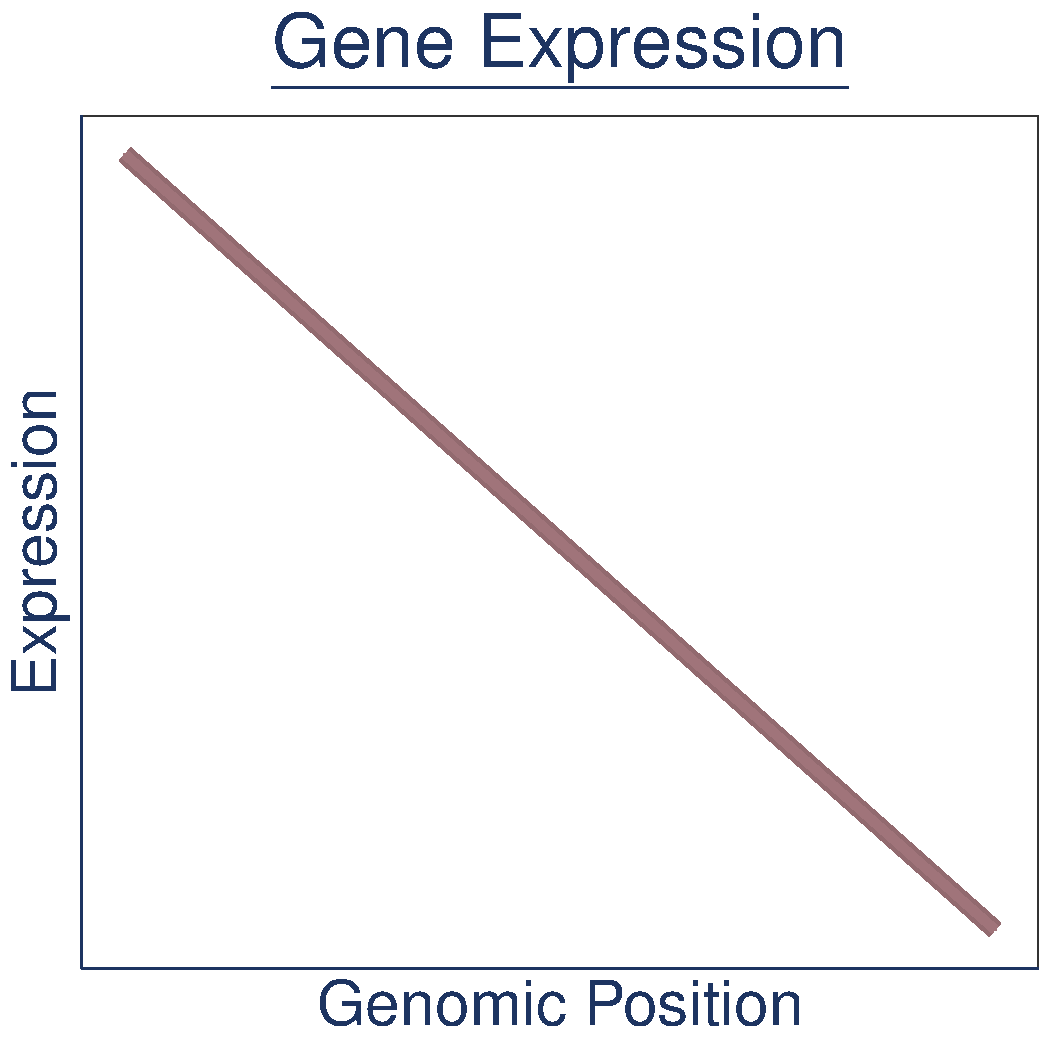
\includegraphics[width=0.67\textwidth]{./exp_graph.pdf}
		\column{.5\textwidth}
		\textbf{Observation: }
		\bigskip 
		
		\textbf{Gene expression decreases} with increasing distance from the origin of replication in a \textbf{non-linear} manner
	\end{columns}
	
	\btVFill
	\tiny \vspace{-\baselineskip}\color{berry}{Couturier et al. 2006, Cooper et al. 2010, Sharp et al. 2005, Morrow et al. 2012, Cooper and Rocha 2006}
	%		\sourceright{Couturier et al. 2006, Cooper et al. 2010, Sharp et al. 2005, Morrow et al. 2012, Cooper and Rocha 2006}
	
\end{frame}

%%%%%%%%%%%%%%%%%%%%%%%%%%%%%%%%%%%%%%%%%%%%%%%%%%%%%%%
\begin{frame}{Selection}
	Measuring what evolutionary forces are acting on genes
	\pause
	\bi
	\itm \textbf{dN} = non-synonymous substitution rate
		\bi
		\itm change in amino acid sequence
		\itm can alter function of the protein
		\ei
		\pause
	\itm \textbf{dS} = synonymous substitution rate
		\bi
		\itm no change in amino acid sequence
		\itm will not alter function of protein
		\ei
		\pause
	\itm \textbf{ $\omega$ = (dN/dS)}
	\pause
		\bi
		\itm \textbf{$\omega$ $>$ 1} $\rightarrow$ positive selection
			\bi
			\itm beneficial to the organism and will likely be maintained over time
			\ei
			\pause
		\itm \textbf{$\omega$ = 1} $\rightarrow$ neutral selection
			\bi
			\itm neither beneficial nor deleterious to the organism
			\ei
			\pause
		\itm \textbf{$\omega$ $<$ 1} $\rightarrow$ negative selection
			\bi
			\itm deleterious to the organism and will likely not be maintained over time
			\ei
		\ei
	\ei
\end{frame}

%%%%%%%%%%%%%%%%%%%%%%%%%%%%%%%%%%%%%%%%%%%%%%%%%%%
\begin{frame}[t]{The Data}
			\textbf{Selection}
			\bi
			\itm \ecol, \bass, \strep, and \smel
			\itm dN, dS, and $\omega$ $+$ distance from the origin of replication
			\itm $\omega$ $>$ 1 (positive selection), $\omega$ = 1 (neutral), $\omega$ $<$ 1 (negative selection)
			\itm \textbf{Expectations:} 
			\begin{enumerate}
				\item dS $>$ dN
				\item Most genes are under neutral or negative selection
				\item Genes that are under positive selection should most likely be accessory genes
			\end{enumerate}
			\bi
			\itm Core genes are near the origin of replication
			\itm Accessory genes are usually near the terminus
			\ei
			\ei
\end{frame}
%%%%%%%%%%%%%%%%%%%%%%%%%%%%%%%%%%%%%%%%%%%%%%%%%%
%%%%%%%%%%%%%%%%%%%%%%%%%%%%%%%%%%%%%%%%%%%%%%%%%%
\begin{frame}{Selection Summary}
	\centering
	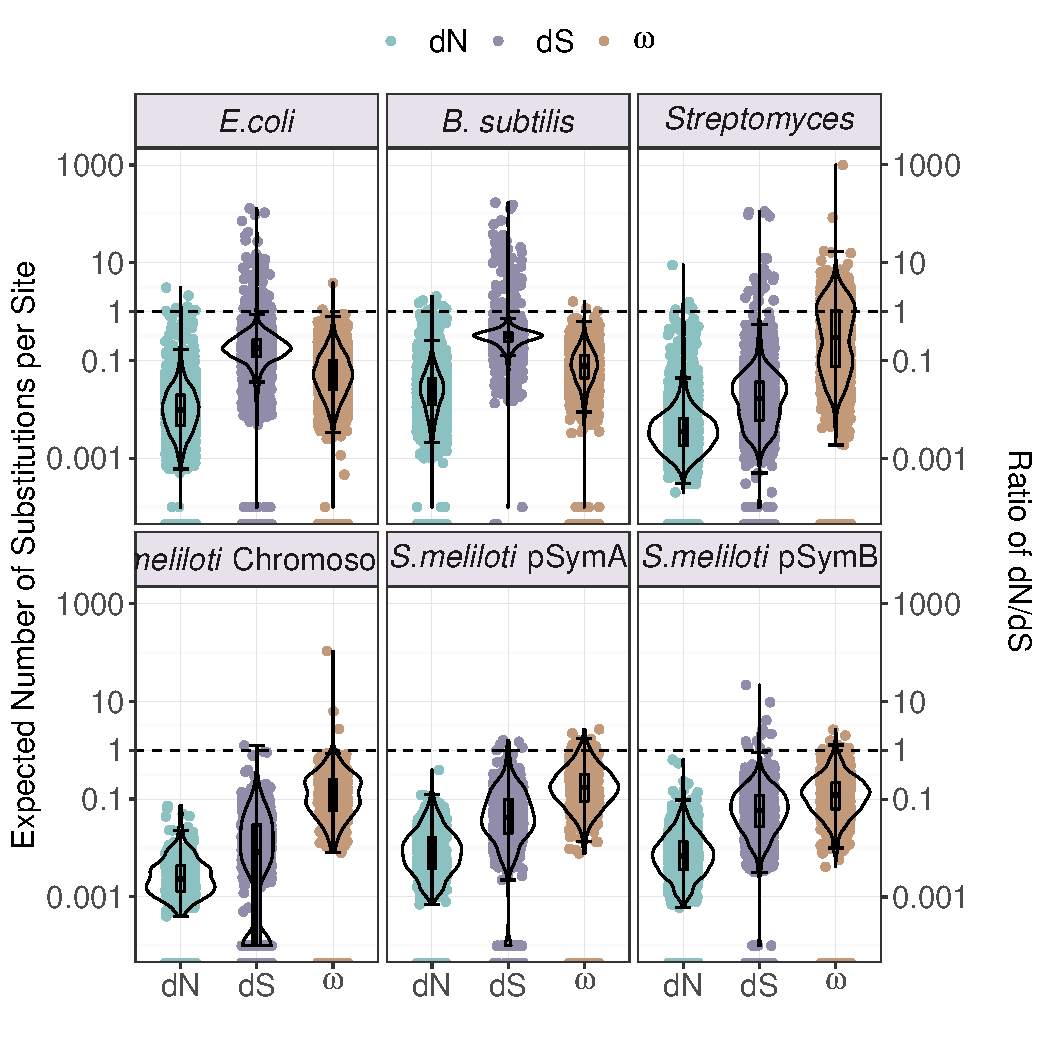
\includegraphics[width=0.8\textwidth]{selection_vio_box.pdf}
\end{frame}
%%%%%%%%%%%%%%%%%%%%%%%%%%%%%%%%%%%%%%%%%%%%%%%%%%
%%%%%%%%%%%%%%%%%%%%%%%%%%%%%%%%%%%%%%%%%%%%%%%%%%
\begin{frame}{\strep Selection}
	\centering
	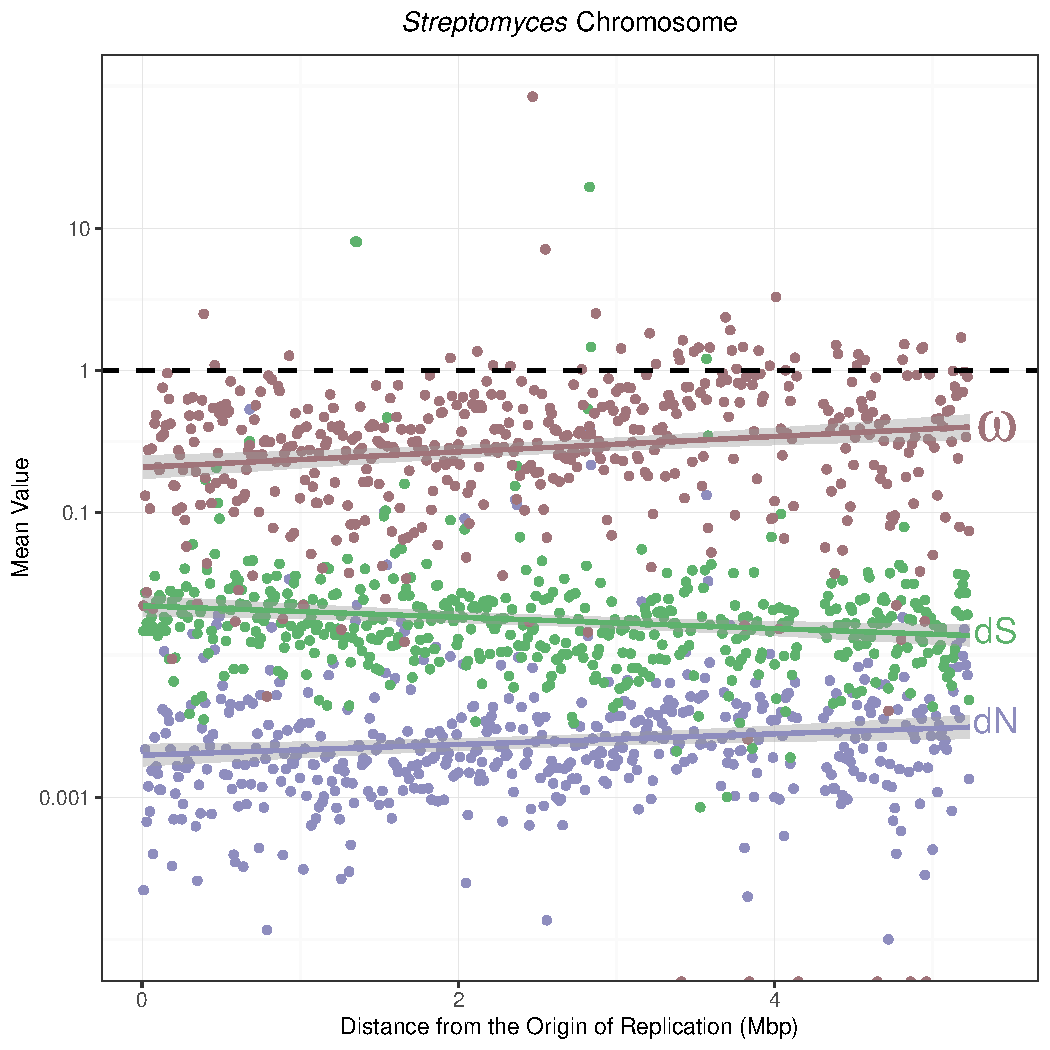
\includegraphics[width=0.77\textwidth]{strep_selection.pdf}
\end{frame}

%%%%%%%%%%%%%%%%%%%%%%%%%%%%%%%%%%%%%%%%%%%%%%%%%%
\begin{frame}{Summary}
	\ch Gene expression decreases (non-linearly) with increasing distance from the origin of replication
	\bi
	\itm  Wave-like pattern at the end of the graph?
	\ei

	\ch dS $>$ dN

	\ch Most genes are under neutral or negative selection ($\omega$ $\le$ 1)

	\ch In \strep, genes under positive selection ($\omega$ $>$ 1) were near the terminus and most likely accessory genome
\end{frame}
%%%%%%%%%%%%%%%%%%%%%%%%%%%%%%%%%%%%%%%%%%%%%%%%%%

\end{document}
